\documentclass{beamer}
\usepackage[utf8]{inputenc}
\usepackage[T1]{fontenc}
\usetheme{Frankfurt}
\usecolortheme{whale}

\title{Git - Die Macht der Versionierung}
\author{Fnordberg}
\date{\today}
\definecolor{git-orange}{RGB}{241, 80, 47}
\setbeamercolor{title}{bg=git-orange}
\setbeamercolor{frametitle}{bg=git-orange}
\setbeamercolor{item}{fg=git-orange}
\setbeamercolor{block title}{bg=black}
\titlegraphic{
\includegraphics[scale=0.20]{pictures/git-logo.png}}
\begin{document}
\maketitle

\section{Einleitung}

\begin{frame}{Was möchte ich mit diesen Vortrag erreichen?}
    \begin{minipage}[b]{80mm}
        \begin{itemize}
            \item einen Einblick geben
            \item die wichtigsten Befehle von Git zeigen
            \item Euch ermutigen Git zu benutzen
        \end{itemize}
    \end{minipage}
            \hfill
    \begin{minipage}[b]{20mm}
        
\includegraphics[width=20mm]{pictures/pic-tux_1.png}
    \end{minipage}
\end{frame}

\begin{frame}{Was möchte ich mit diesen Vortrag 
                    \textbf{nicht} erreichen?}
                    
    \begin{minipage}[b]{80mm}
        \begin{itemize}
            \item Euch bekehren
            \item eine Allumwassende Einführung geben
        \end{itemize}
    \end{minipage}
        \hfill
    \begin{minipage}[b]{20mm}
         
\includegraphics[width=20mm]{pictures/pic-tux_2.png}
    \end{minipage}

\end{frame}

\begin{frame}{Ohne Versions Kontrolle Systeme} 

-rw-r--r-- 1 fnordberg fnordberg 0 May 23 23:42 arbeit$\_$v1.pdf
-rw-r--r-- 1 fnordberg fnordberg 0 Jun 12 13:31 arbeit$\_$v2.pdf
-rw-r--r-- 1 fnordberg fnordberg 0 Jun 17 09:34 arbeit$\_$v3.pdf

\end{frame}

\begin{frame}{es geht aber auch noch schlimmer...}

-rw-r--r-- 1 fnordberg fnordberg 0 May 23 23:42 arbeit$\_$alt.pdf
-rw-r--r-- 1 fnordberg fnordberg 0 Jun 12 13:31 arbeit$\_$neu.pdf
-rw-r--r-- 1 fnordberg fnordberg 0 Jun 17 09:34 arbeit$\_$neuer.pdf
-rw-r--r-- 1 fnordberg fnordberg 0 Jun 23 12:38 arbeit$\_$neuer(1).pdf

\end{frame}

\begin{frame}{Versions Kontroll Systeme}
    
    \begin{itemize}
        \item Lokales System
        \item Zentralisiertes System
        \item Verteiltes System
    \end{itemize}
\end{frame}
\begin{frame}{wie macht Git das?}
 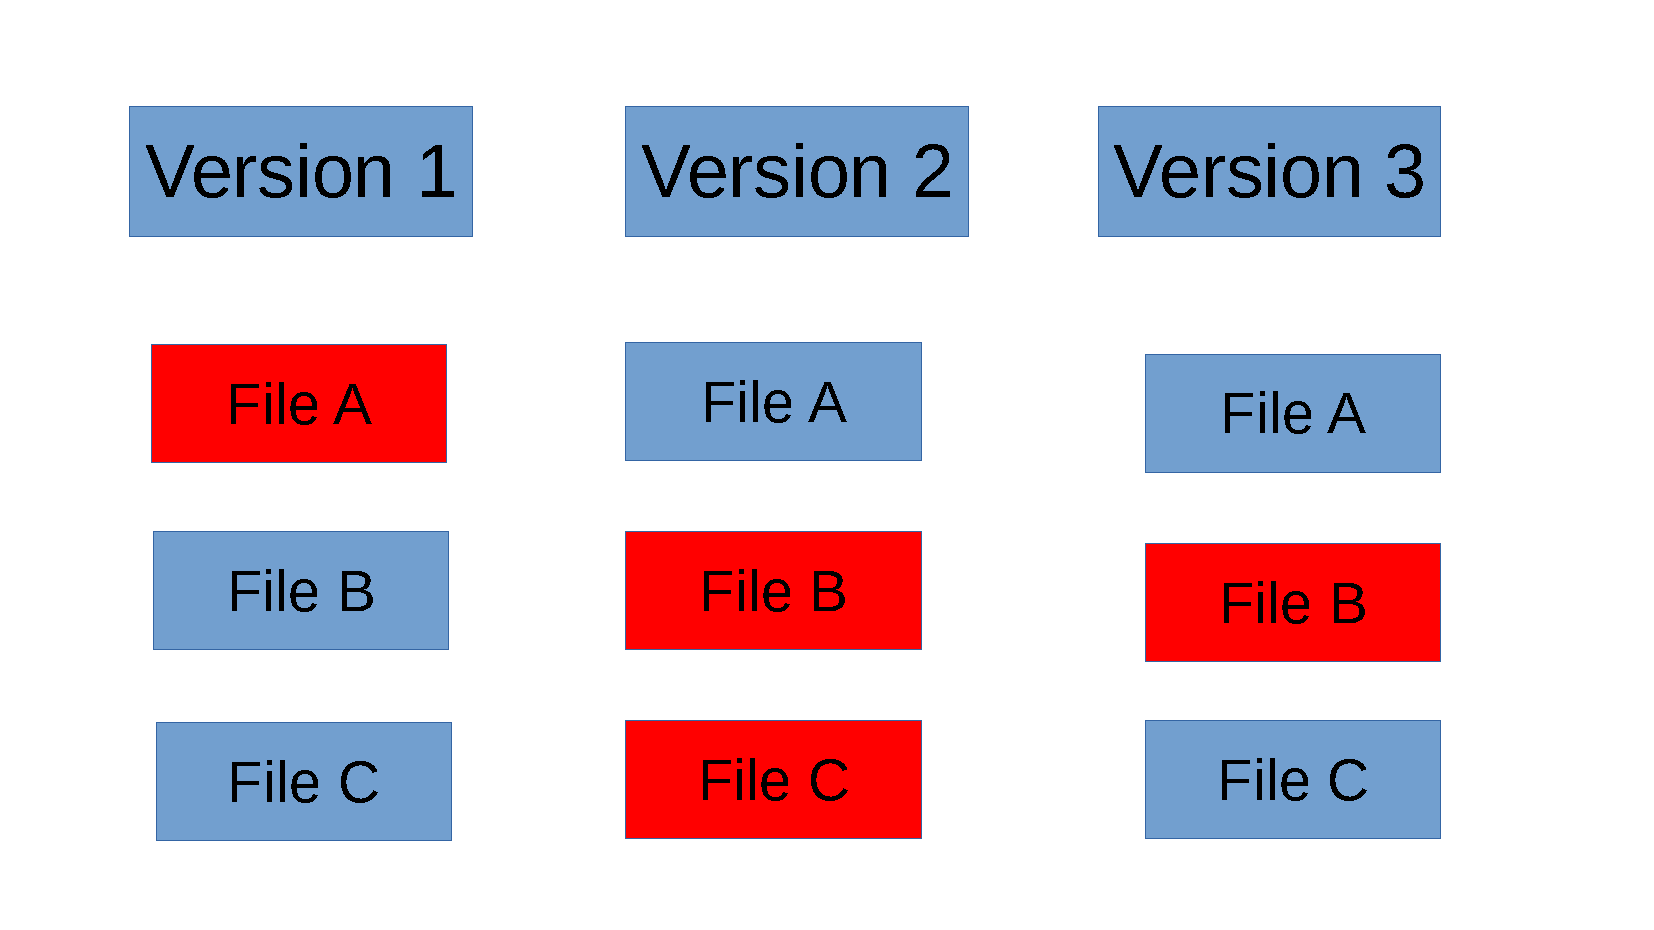
\includegraphics[scale=0.5]{pictures/git-versionen.pdf}   
\end{frame}


\section{Git - die Geschichte}

\begin{frame}{Git - die Geschichte}
   
    \begin{itemize}
        \item Verwaltung des Linux Kernels
        \item ab 2002 wurde der Kernel mit Bitkeeper verwaltet
            \begin{itemize}
                \item ist kostenflichtig - 
                \item wurde aber von Bitkeeper kostenlos gestellt
            \end{itemize}
        \item 2005 kam es jedoch zum Bruch mit Bitkeeper
        \item 2005 wurde das Versionierungstool Git von Linus Torvalds geschrieben
    \end{itemize}

\end{frame}

\begin{frame}{Anforderung an Git}
    
    \begin{itemize}
        \item Verteiltes Versions Kontroll System
        \item Schnell
        \item Einfach
        \item mit großen Datenmengen umgehen können
        \begin{itemize}
         \item z.B. der Windows Kernel wird mit Git versoniert
         \item der Linux Kernel natürlich auch
        \end{itemize}
        \item nicht lineare Entwicklung unterstützen
    \end{itemize}

\end{frame}

\begin{frame}{Git wird geboren - 2005}

Git ist englisch und heißt sowas wie Trottel oder Blödmann. \newline \newline

  \begin{quote}
    „Ich bin ein egoistischer Mistkerl, und ich benenne all meine Projekte nach mir. Zuerst ‚Linux‘, jetzt eben ‚Git‘.“  \\
    - Linus Torvalds
  \end{quote}
  
\end{frame}

\begin{frame}{Die Wahrheit}
     \begin{quote}
        „Der Witz ‚Ich benenne alle meine Projekte nach mir, zuerst Linux, nun eben Git‘ war einfach zu gut, um ihn nicht zu machen. 
        Aber es (der Befehl) ist auch kurz, einfach auszusprechen und auf einer Standardtastatur zu schreiben, dazu einigermaßen 
        einzigartig und kein gewöhnliches Standardkommando – sehr ungewöhnlich.“ \\
	    – Linus Torvalds
     \end{quote}

\end{frame}

\section{Praktisches}

\begin{frame}{Git installieren}
    
    \begin{block}{Debian basierte}
        sudo apt install git
    \end{block}
    
    \begin{block}{Arch basierte}
        sudo pacman -S git
    \end{block}
    
    \begin{block}{RPM basierte}
         sudo dnf install git-all  
    \end{block}
    
    \begin{block}{OpenSuse}
        sudo zypper in git-core       
    \end{block}

\end{frame}

\begin{frame}{Git konfigurieren}
    
    git config $- -$ global user.name „Fnordberg“ \\
    git config $- -$ global user.email „Fnordberg@posteo.org“ 
    \newline
    \newline
    man kann mit config auch Shortcuts anlegen aber das geht zuweit
    
\end{frame}

\begin{frame}{Ein Repository erstellen}
    
    \begin{block}{Repository installieren}
     git init
    \end{block}
    
    \begin{block}{Status abfragen}
     git status
    \end{block}
    
\end{frame}

\begin{frame}{Github/Gitlab}
    \begin{itemize}
         \item Versionierungs Kontroll System Server
         \item Server für Git Anwendungen
         \item werden von Software Projekte benutzt
         \item kann aber auch Privat genutzt werden
    \end{itemize}
\end{frame}

\begin{frame}{Github}
    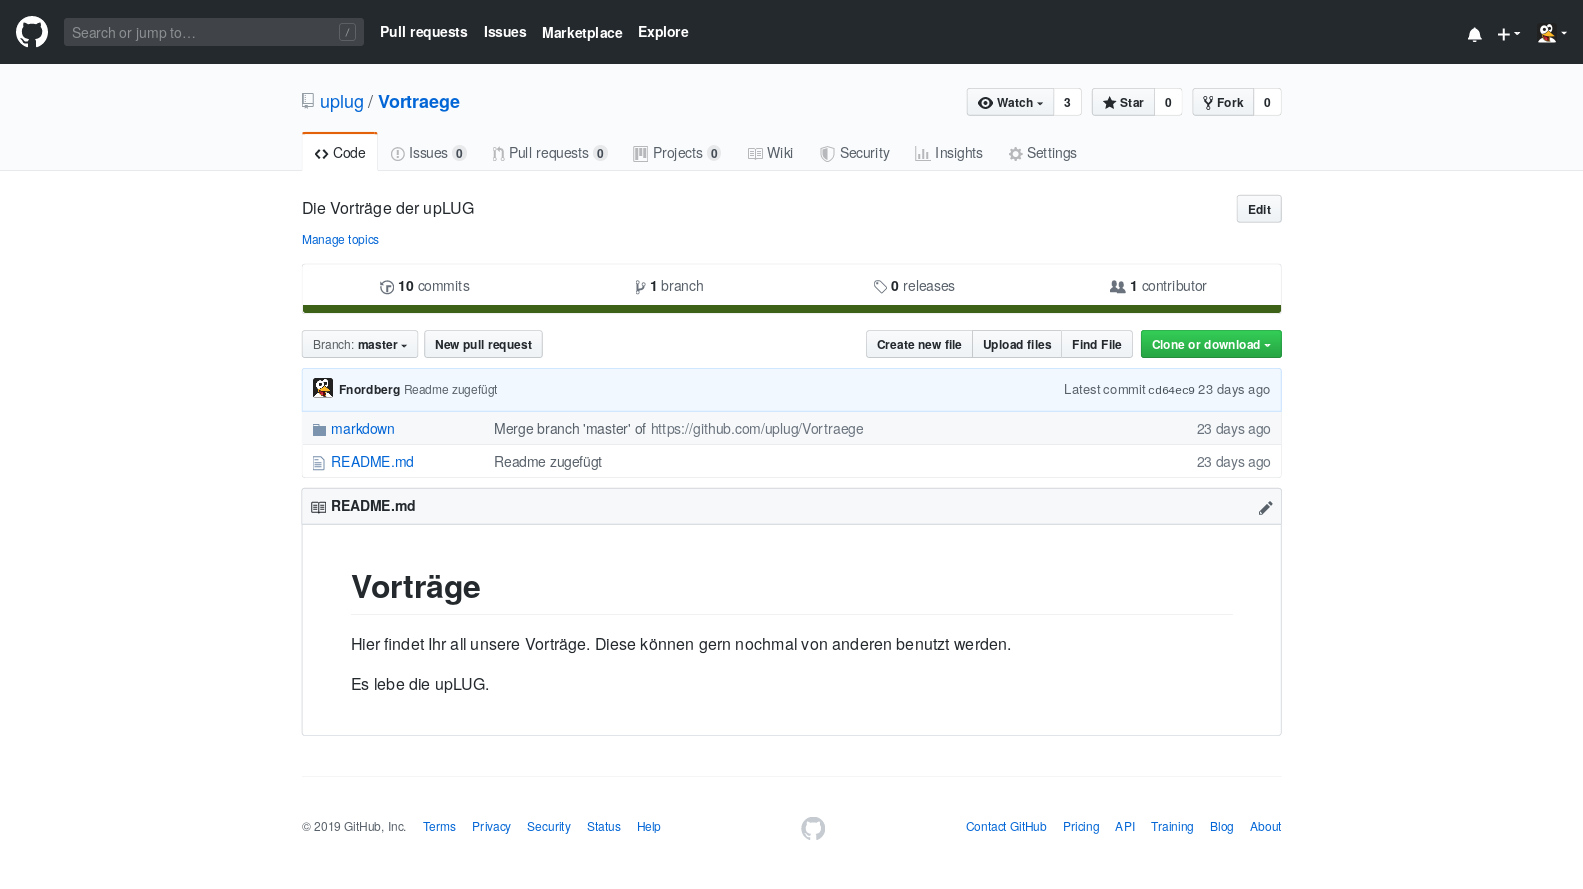
\includegraphics[scale=0.20]{pictures/github.png}
\end{frame}{}

\begin{frame}{Ablauf}
    \begin{minipage}[b]{70mm}
 
 git clone https://github.com/uplug/Werbematerial.git \\
 \newline
 *Dinge ändern an file A.txt* \\
 \newline
 git add A.txt \\
 \newline
 git commit -m "Was verändert wurde"  \\
 \newline
 git push \\
    \end{minipage}
            \hfill      
    \begin{minipage}[b]{30mm}
        
\includegraphics[width=30mm]{pictures/tower.png}
    \end{minipage}
\end{frame}

\begin{frame}{Ablauf}
    \begin{minipage}[b]{70mm}
 
 git pull \\
 \newline
 *Dinge ändern an allen Files ändern* \\
 \newline
 git add . \\
 \newline
 git commit -m "Änderungen" \\
 \newline
 git push \\
    \end{minipage}
            \hfill    
    \begin{minipage}[b]{30mm}
        
\includegraphics[width=30mm]{pictures/laptop.png}
    \end{minipage}
\end{frame}

\section{Visualisierung}

\begin{frame}{git init}
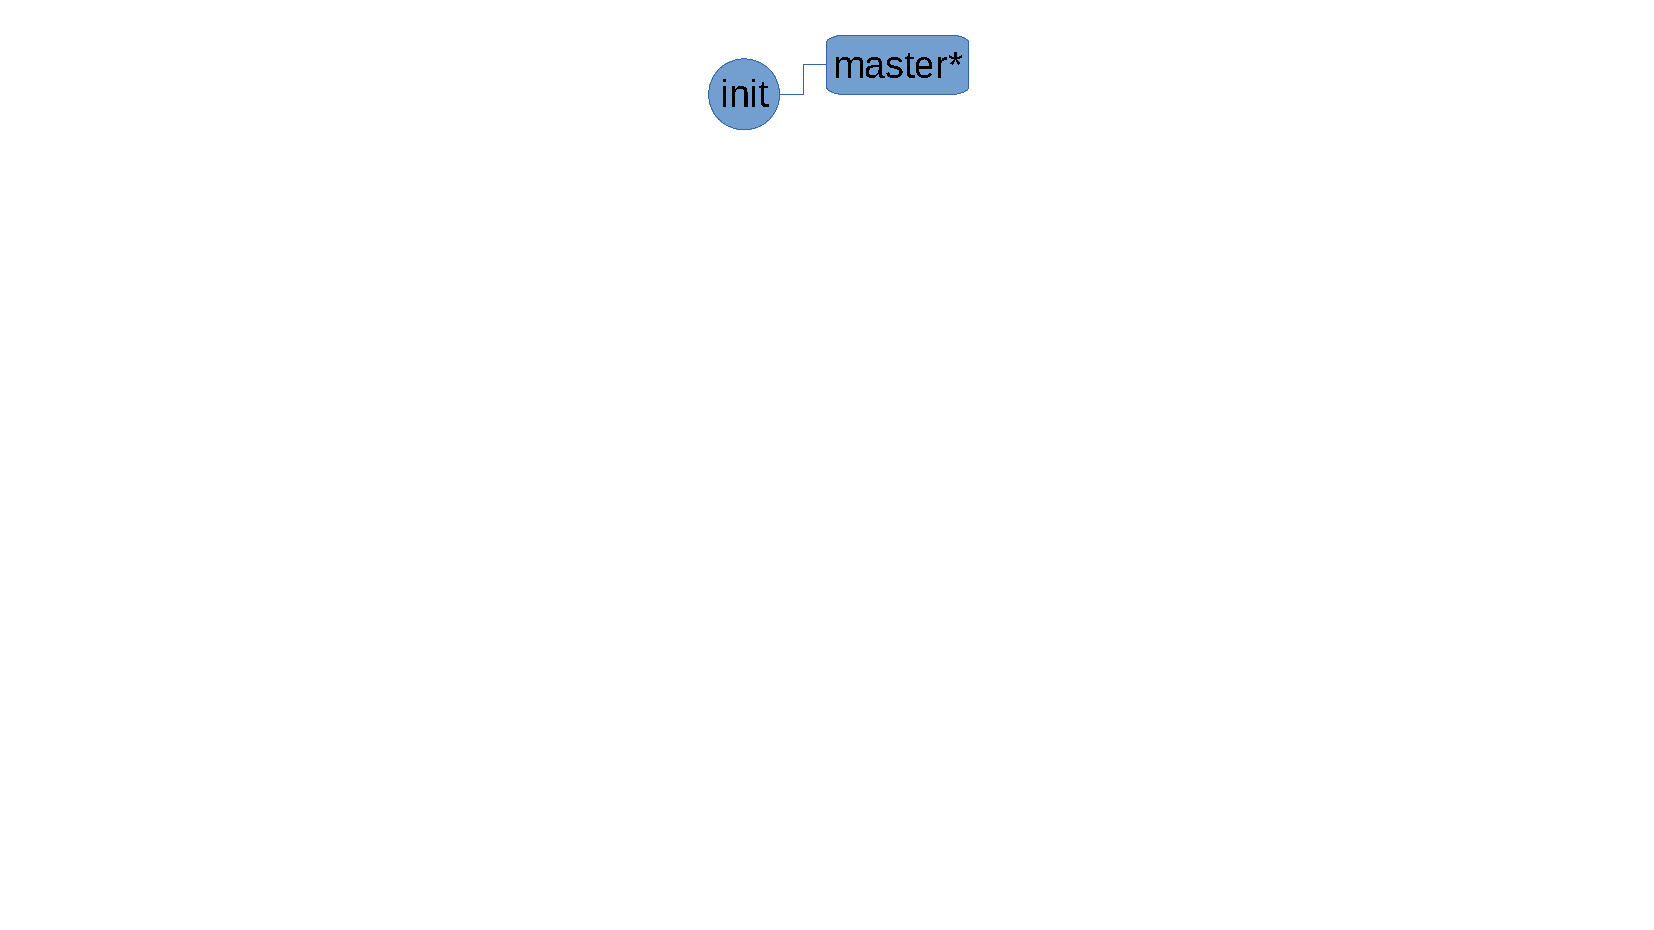
\includegraphics[scale=0.5]{pictures/init.pdf}
\end{frame}

\begin{frame}{git commit -m "erstes commit"}
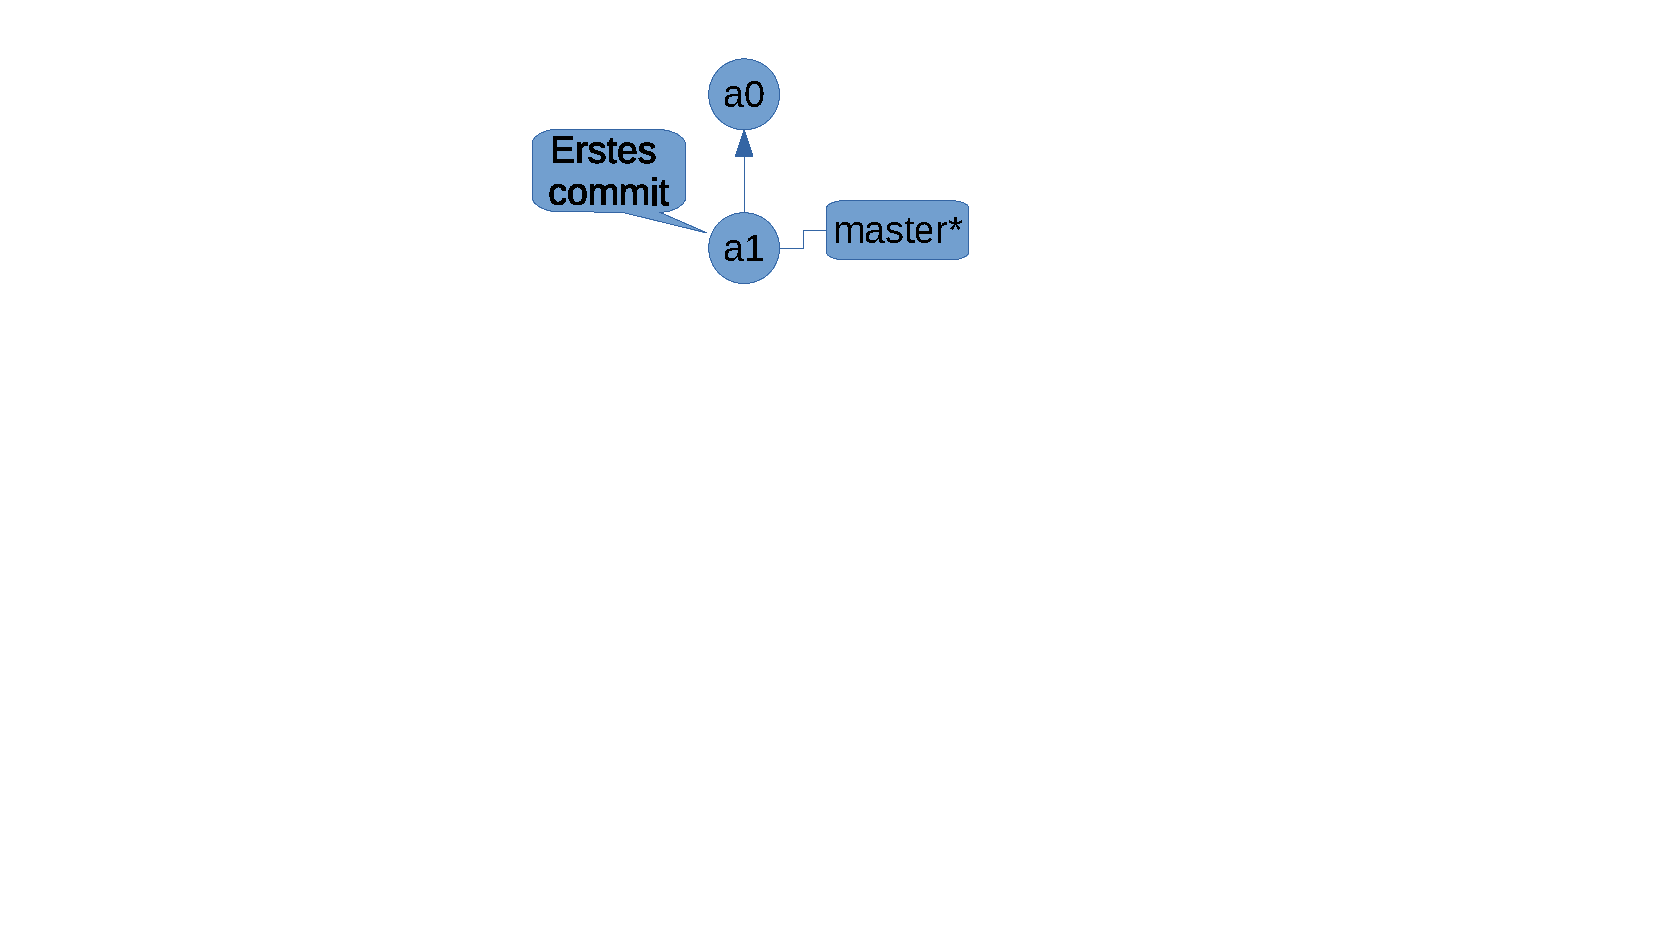
\includegraphics[scale=0.5]{pictures/first_commit.pdf}
\end{frame}

\begin{frame}{git commit -m "zweites commit"}
    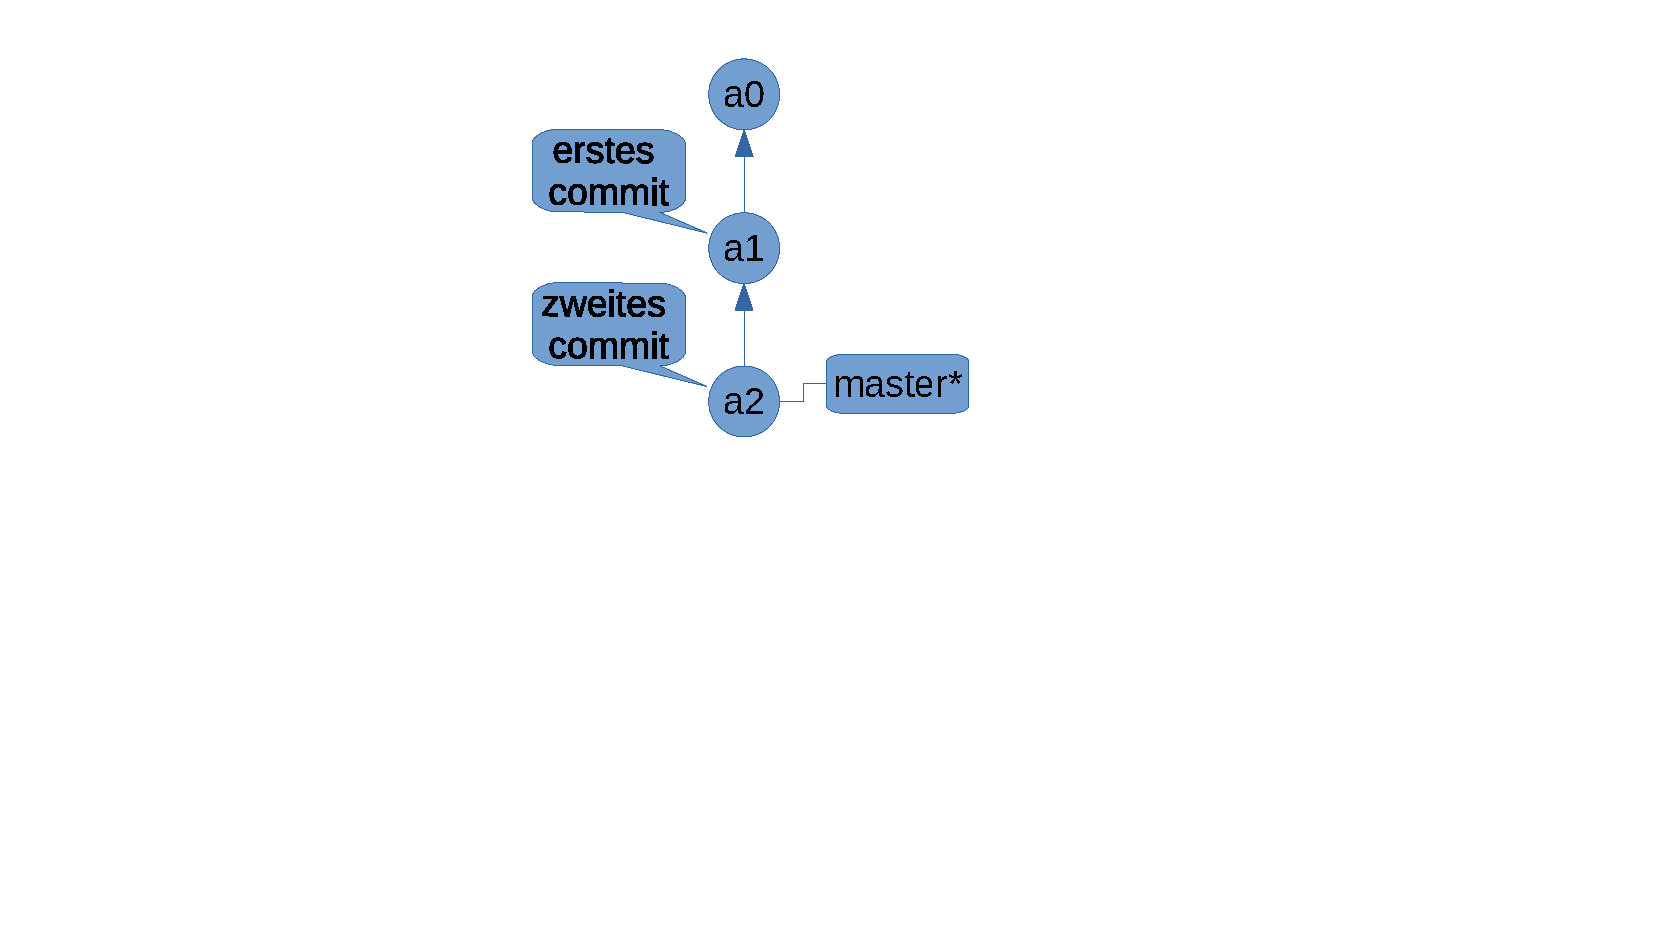
\includegraphics[scale=0.5]{pictures/second_commit.pdf}
\end{frame}

\begin{frame}{git branch versuch}
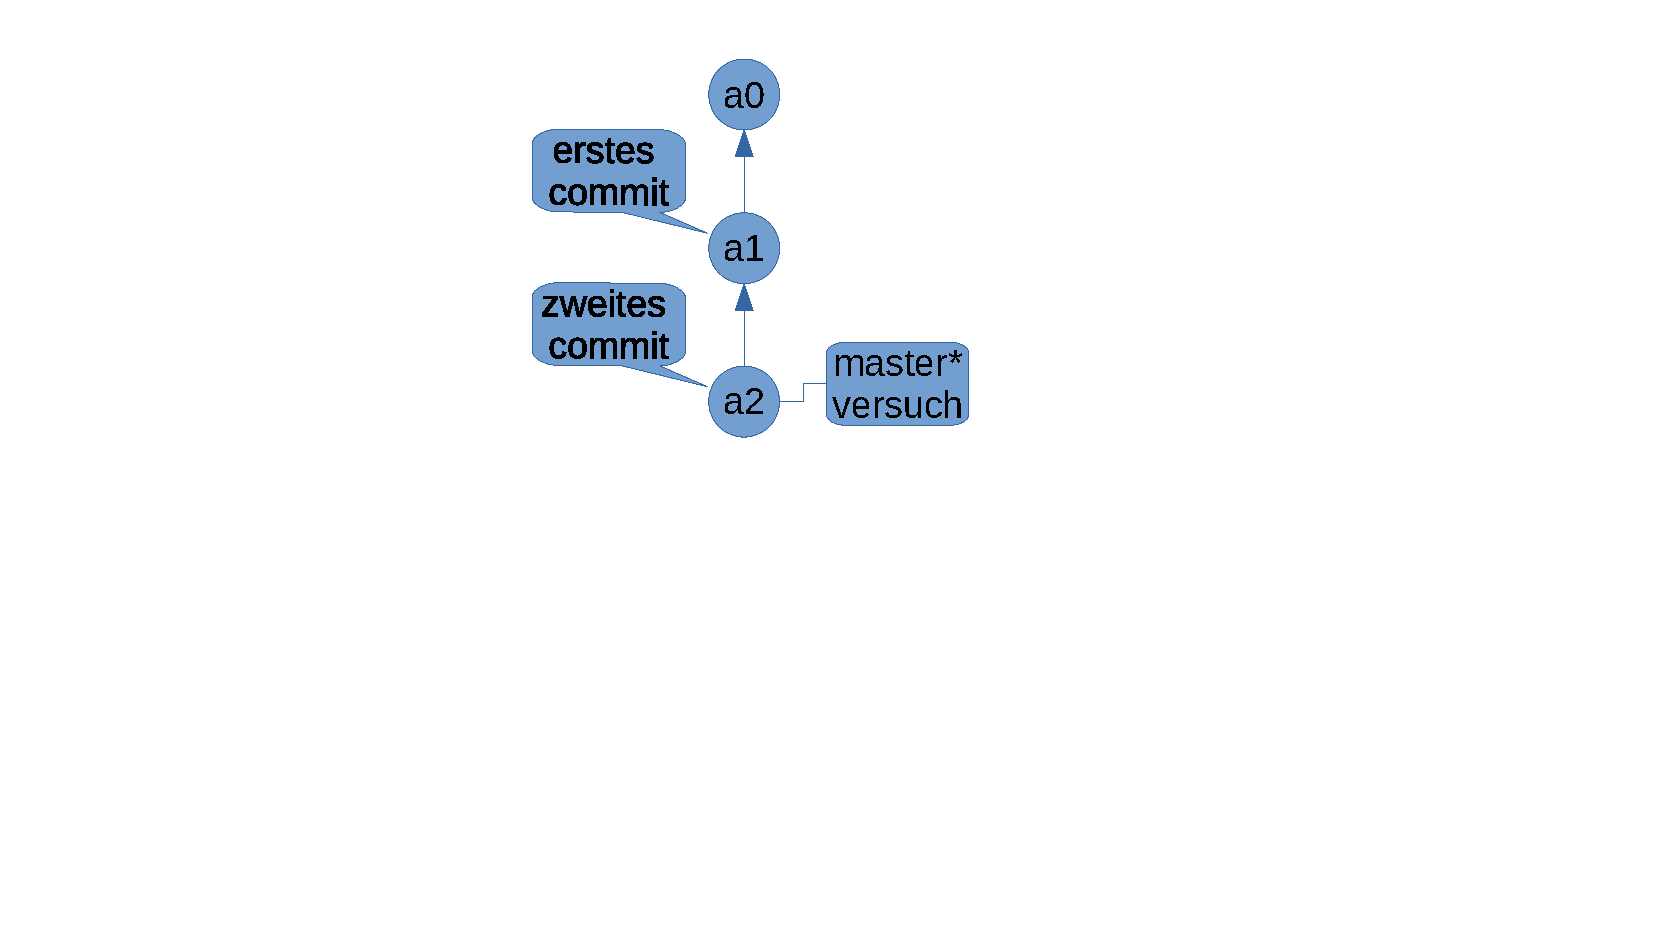
\includegraphics[scale=0.5]{pictures/branch.pdf}
\end{frame}

\begin{frame}{git commit -m  "drittes commit"}
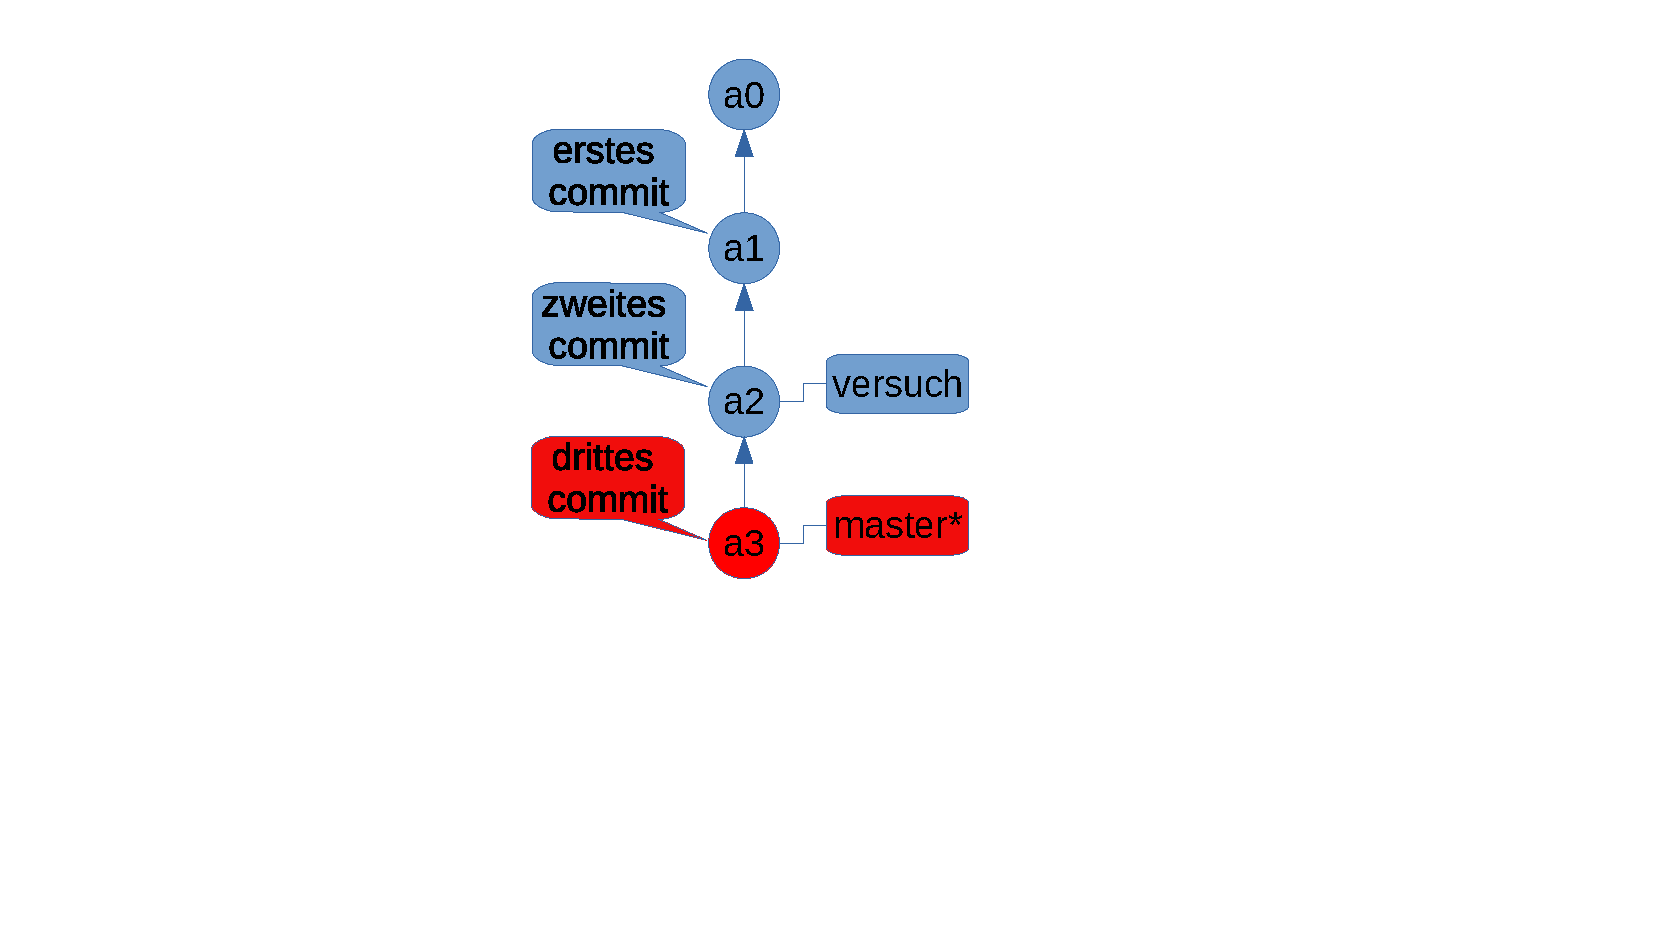
\includegraphics[scale=0.5]{pictures/third_commit.pdf}
\end{frame}

\begin{frame}{git checkout versuch}
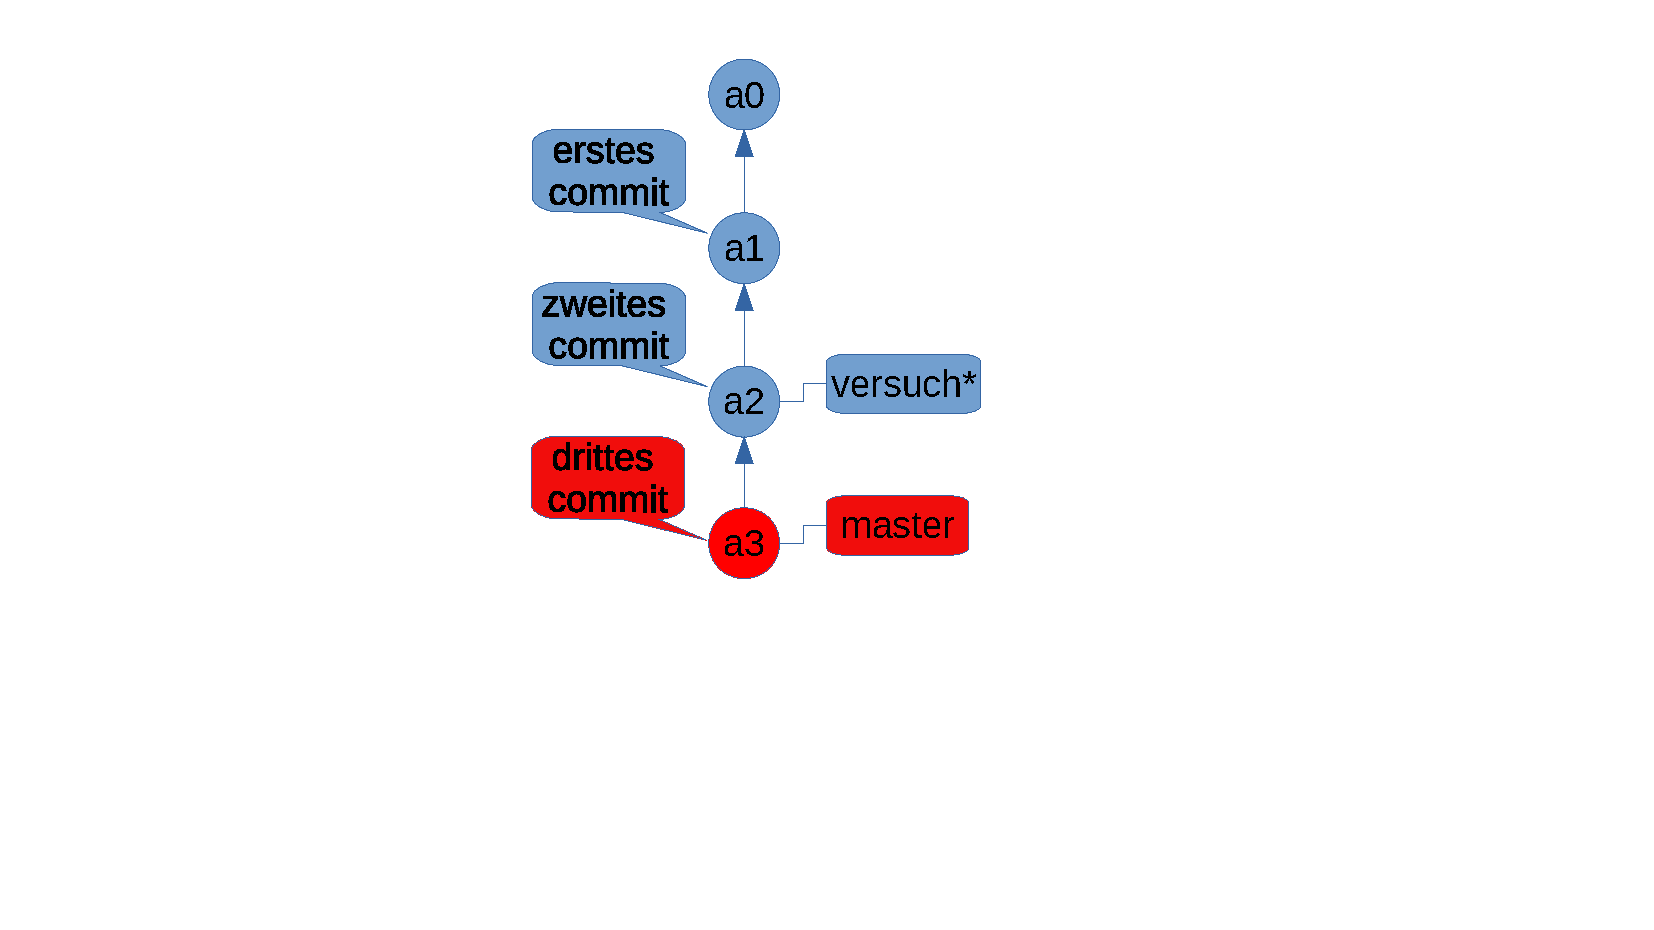
\includegraphics[scale=0.5]{pictures/checkout.pdf}
\end{frame}

\begin{frame}{git commit -m "viertes commit"}
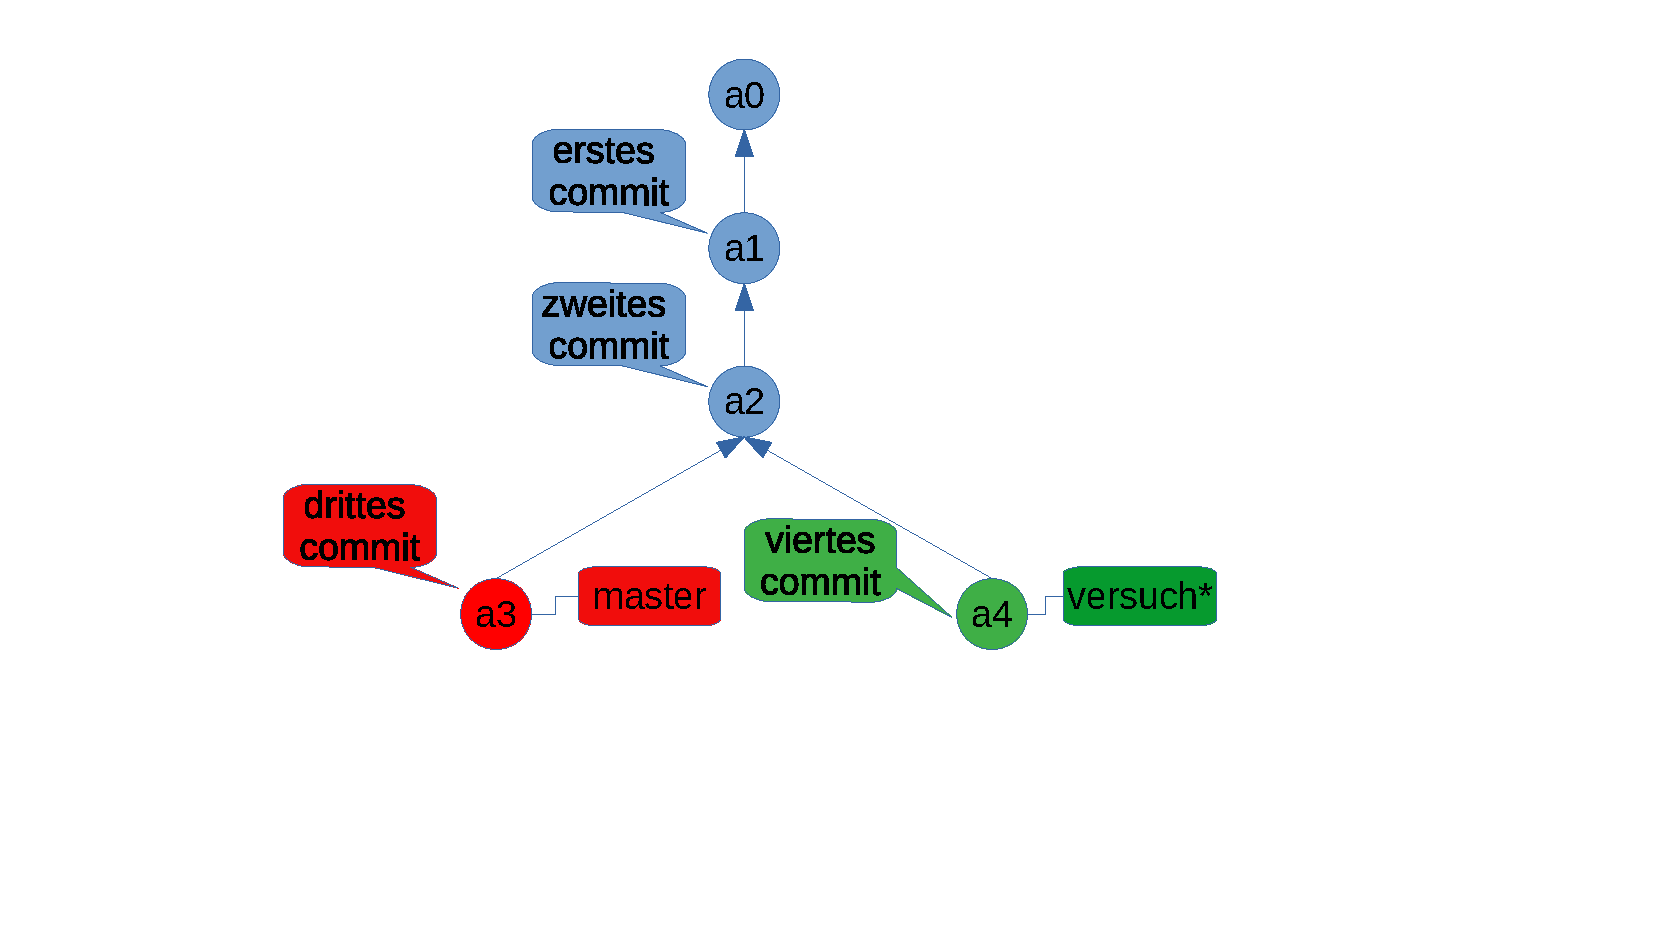
\includegraphics[scale=0.5]{pictures/forth_commit.pdf}
\end{frame}

\begin{frame}{git merge master}
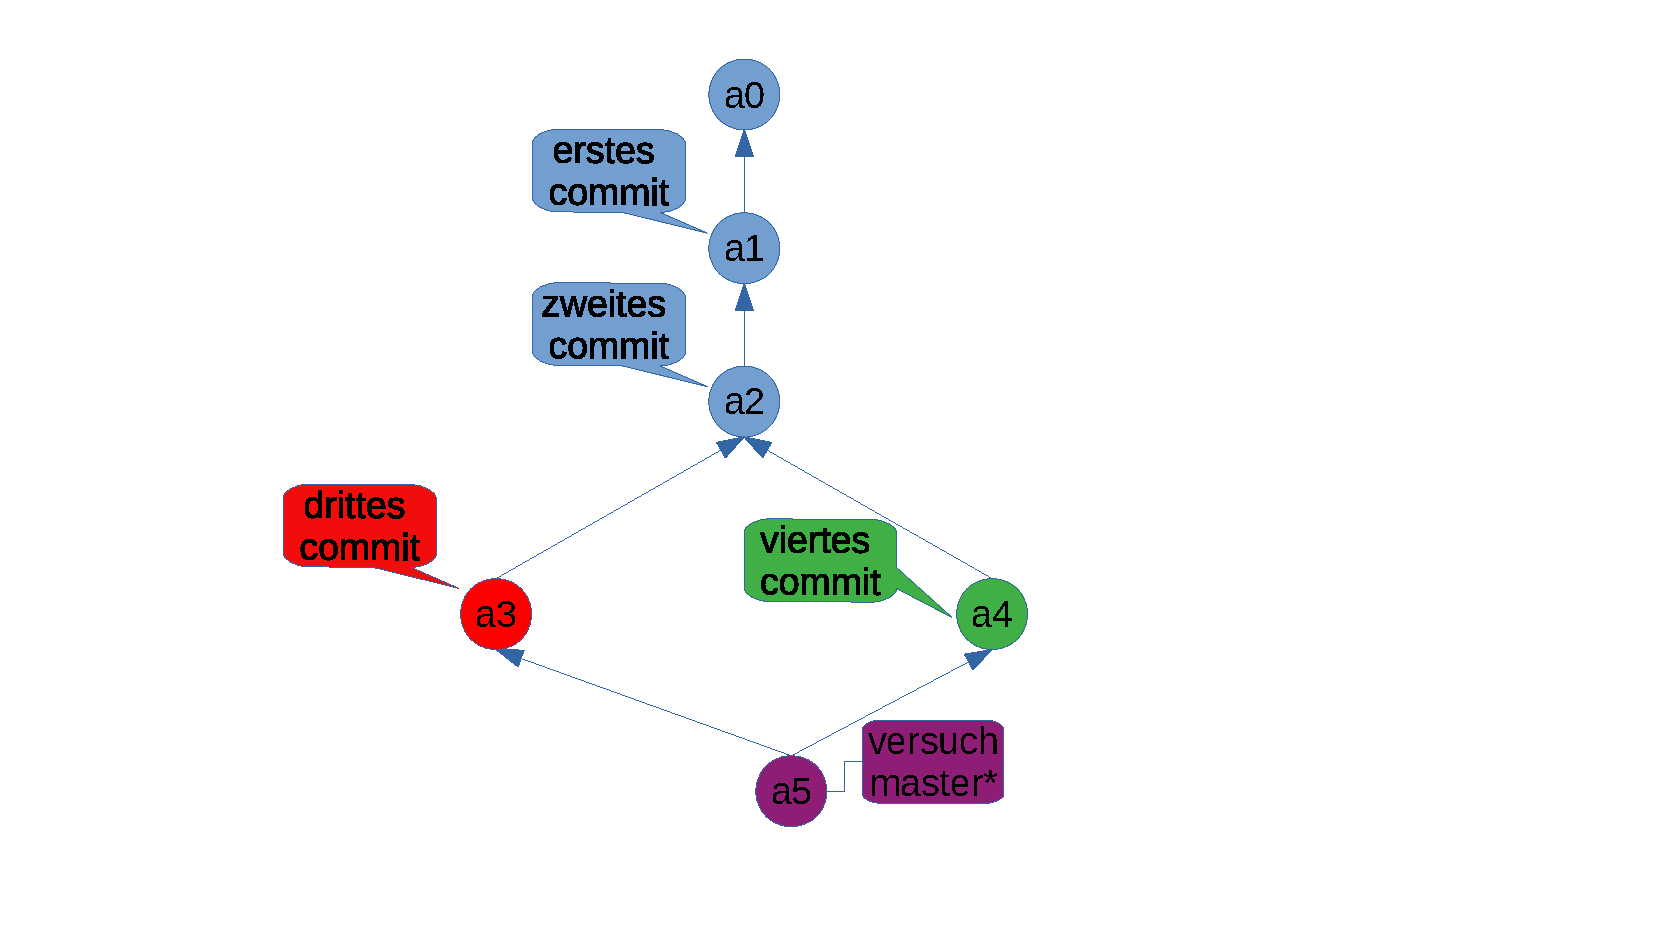
\includegraphics[scale=0.5]{pictures/merge.pdf}
\end{frame}

\begin{frame}{git log}
commit 694d7f632ee8dcefc1d80392e84b13067225f7a9 \\
Author: Fnordberg <lllllllllllll@posteo.org> \\
Date:   Fri May 31 15:30:12 2019 +0200 \\
    Asta Logo und Impressum \\
commit 6251862e7faacff4e1cd13d0d3484d5ea4ccf3cf \\
Author: Fnrodberg <lllllllllllll@posteo.org> \\
Date:   Tue May 28 16:13:48 2019 +0200 \\

    Zwei neue Poster zugefügt
\end{frame}

\begin{frame}{git checkout a1}
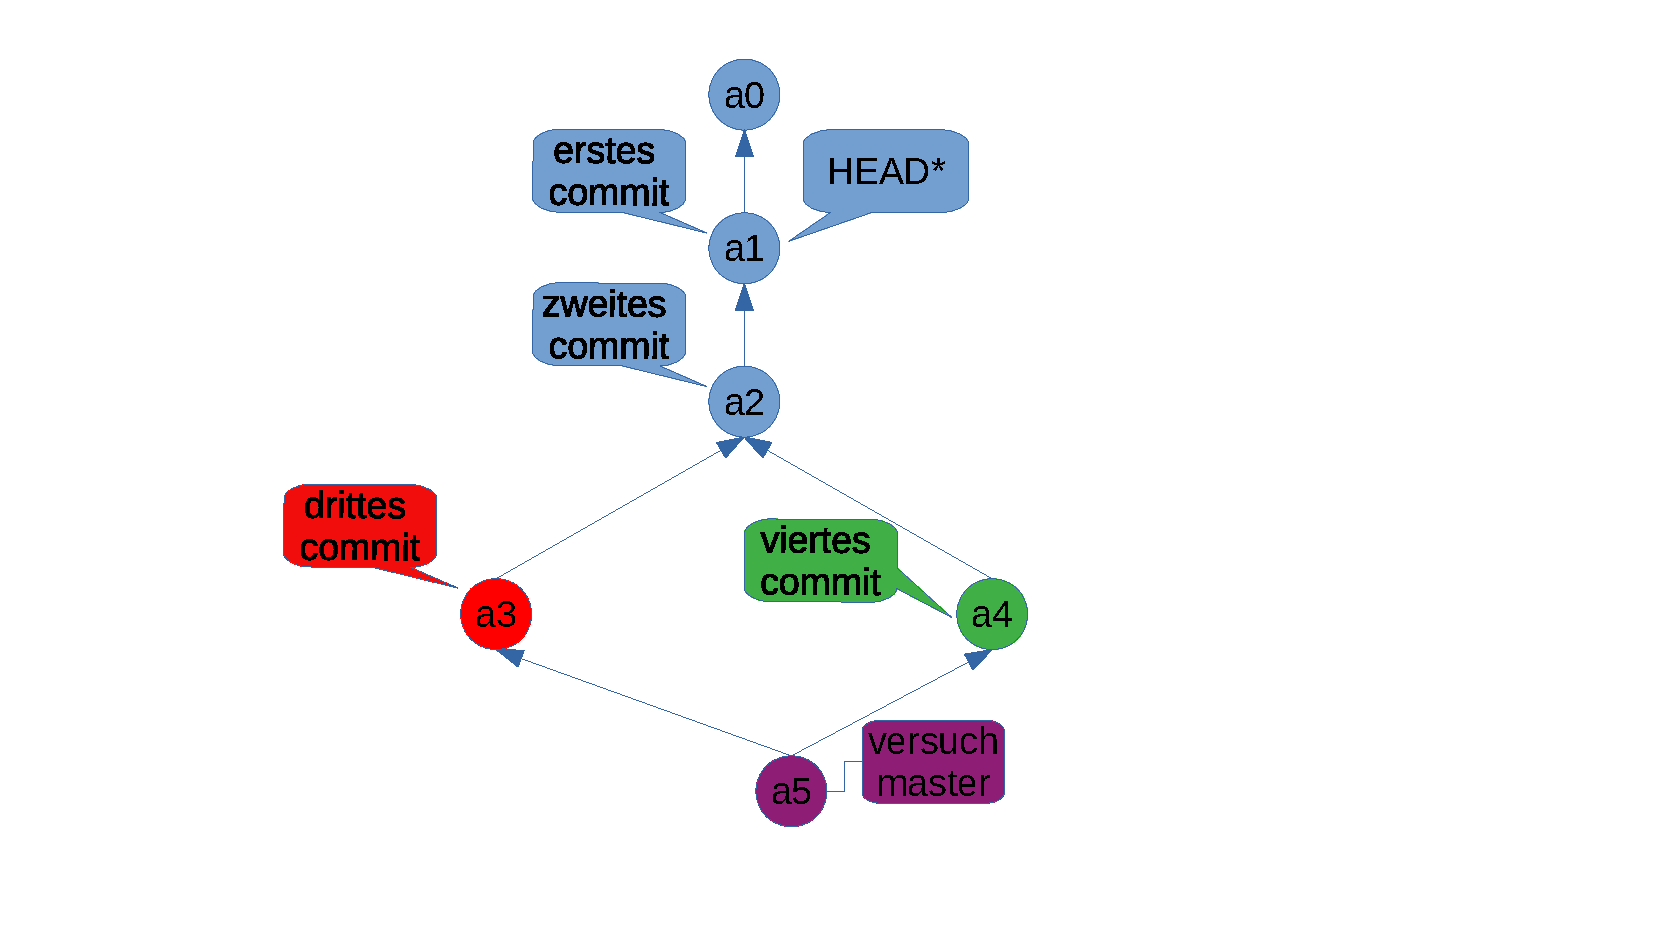
\includegraphics[scale=0.5]{pictures/checkout_a1.pdf}
\end{frame}


\begin{frame}{Vielen Dank!}
    
\includegraphics[scale=0.17]{pictures/questions.jpg}
\end{frame}

\end{document}
